\documentclass[xcolor=table,slidestop,compress,mathserif]{beamer}
\beamertemplatenavigationsymbolsempty
%\usepackage[no-math]{fontspec}
%\usepackage{xeCJK}
%\setCJKmainfont[BoldFont={Adobe Heiti Std}]{Adobe Song Std}
%\punctstyle{kaiming}
\usepackage{amssymb}
\usepackage{media9}
\usepackage{multimedia}
% setup tikz 
\usepackage{tikz}
\usetikzlibrary{shapes.geometric, arrows}
\tikzstyle{arrow} = [thick,->,>=stealth]
\tikzstyle{roundRec} = [rectangle, rounded corners, minimum width=2cm, minimum height=1cm,text centered, draw=black]
\DeclareGraphicsExtensions{.pdf,.eps,.png,.jpg,.jpeg}

\setbeamertemplate{items}[circle]
\usetheme{Warsaw}
\setbeamertemplate{headline}{}
\defbeamertemplate*{footline}{shadow theme}
{%
  \leavevmode%
  \hbox{\begin{beamercolorbox}[wd=.5\paperwidth,ht=2.5ex,dp=1.125ex,leftskip=.3cm
      plus1fil,rightskip=.3cm]{author in head/foot}%
    \usebeamerfont{author in
      head/foot}\insertshortinstitute\hfill\insertshortauthor
  \end{beamercolorbox}%
  \begin{beamercolorbox}[wd=.5\paperwidth,ht=2.5ex,dp=1.125ex,leftskip=.3cm,rightskip=.3cm
    plus1fil]{title in head/foot}%
    \usebeamerfont{title in
      head/foot}\hfill\insertframenumber\,/\,\inserttotalframenumber%
  \end{beamercolorbox}}%
  \vskip0pt%
}
\usepackage{graphicx}

\pgfdeclareimage[height=0.618cm]{logo}{figures/sjtulogoblue.png}
\logo{\pgfuseimage{logo}}

\def\hilite<#1>{%
  \temporal<#1>{\color{gray}}{\color{blue}}%
  {\color{blue!25}}}
% ------------------------------------------
\title{Audio Event Detection for \\ Automatic Scene Recognition}
\author{Xun Xu}
\institute[CS SJTU]{Department of Computer Science and Engineering \\ Shanghai
  Jiao Tong University}
\date{\today}
\begin{document}
\frame{\titlepage}

% show the outline 
\begin{frame}<beamer>[shrink=10]{Outline}
  \tableofcontents[sectionstyle=show,subsectionstyle=hide]
\end{frame}

% show outline when switch sections
\AtBeginSection[]{
  \begin{frame}<trans|beamer>[shrink=25]{Outline}
    \tableofcontents[sectionstyle=show/shaded,subsectionstyle=show/show/hide]
  \end{frame}
}

% ------------------------------------------

\section{Introduction}
\subsection{Problem Description}
\begin{frame}
  \frametitle{Problem Description}
	In this project, our problem is to recognize a scene where an audio is recorded. 
	Sound example: \\ 
	
	\sound[label=show1, inlinesound]{}{show.wav}
	\hyperlinkmovie[start=0s]{show1}{\beamerbutton{Play Sound}} \\

	%waveform 
	\pause
	\vspace{0.5cm}
	\begin{columns}[c]
		\begin{column}{0.5\textwidth}
			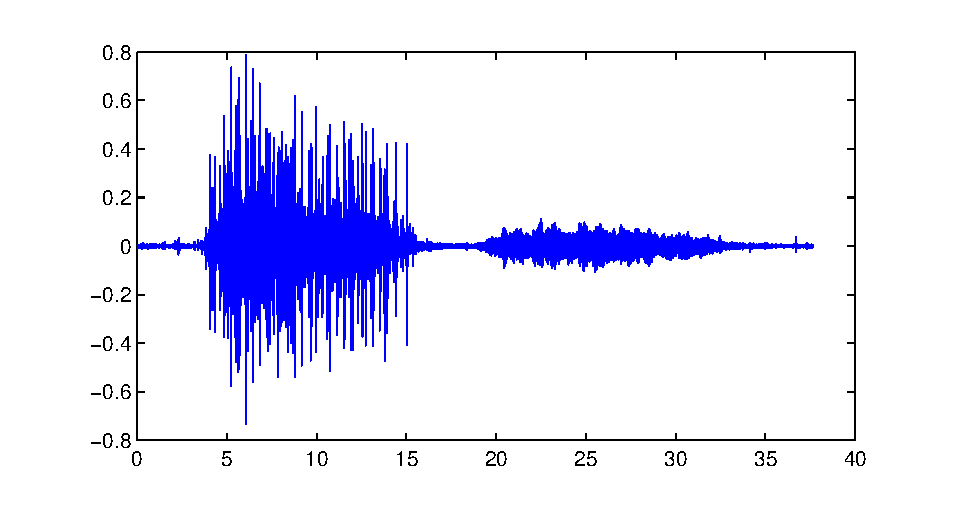
\includegraphics[scale=0.4]{./figure/tune_part.eps}
		\end{column}
		\begin{column}{0.05\textwidth}
			\centering
			$\Rightarrow$
		\end{column}
		\begin{column}{0.45\textwidth}
			\em{concert}
		\end{column}
	\end{columns}

\end{frame}
% ------------------------------------------
\subsection{Approach}
\begin{frame}
  \frametitle{Our Approach}
	Our approach is to detect the audible events in a clip. \\
	Then infer the scene from the detected events. 	
		
	\pause
	\vspace{0.5cm}
	\begin{columns}[c]
		\begin{column}{0.5\textwidth}
			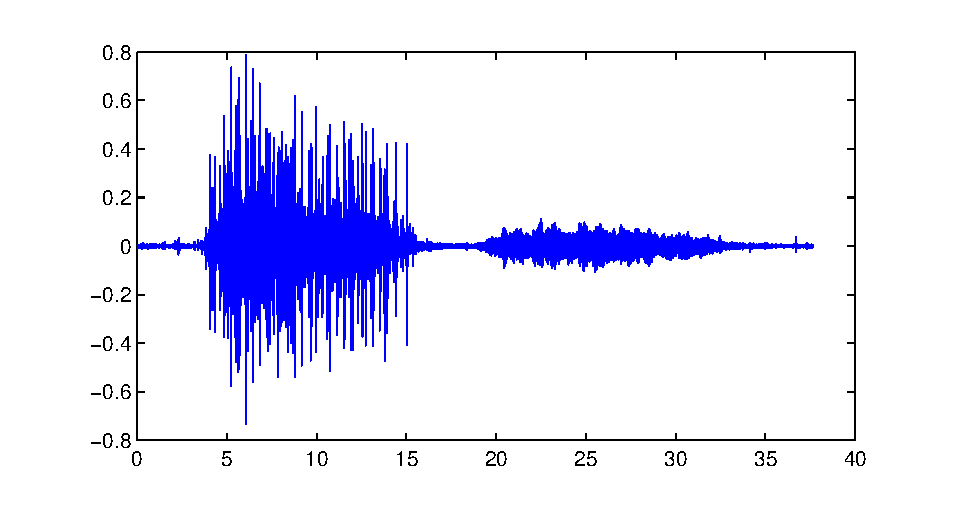
\includegraphics[scale=0.4]{./figure/tune_part.eps}
		\end{column}
		\begin{column}{0.05\textwidth}
			$\Rightarrow$
		\end{column}
		\begin{column}{0.2\textwidth}
			\em{applause, instrument}
		\end{column}
		\begin{column}{0.05\textwidth}
			$\Rightarrow$
		\end{column}
		\begin{column}{0.2\textwidth}
			\em{concert}
		\end{column}
	\end{columns}

\end{frame}
% ------------------------------------------
\begin{frame}
	\frametitle{Our Approach vs. Other Approaches}
	\begin{columns}[c]
		\begin{column}{0.5\textwidth}
			Our approach:
			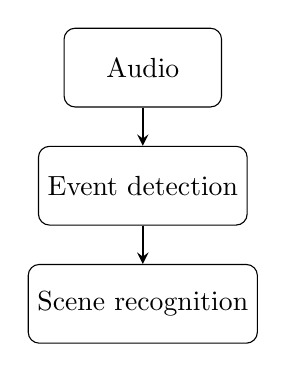
\begin{tikzpicture}[node distance=1.5cm]
				\node (audio) [roundRec] {Audio}; 
				\node (event) [roundRec, below of=audio] {Event detection}; 
				\node (scene) [roundRec, below of=event] {Scene recognition}; 
				\draw [arrow] (audio) -- (event);
				\draw [arrow] (event) -- (scene); 
			\end{tikzpicture}
		\end{column}
		\begin{column}{0.5\textwidth}
			Other approaches:
			\begin{tikzpicture}[node distance=1.5cm]
				\node (audio) [roundRec] {Audio}; 
				\node (scene) [roundRec, below of=event] {Scene recognition}; 
				\draw [arrow] (audio) -- (scene);
			\end{tikzpicture}
		\end{column}
	\end{columns}

\end{frame}
% ------------------------------------------
\section{Audio Event Detection}
\subsection{Audible Event Taxonomy}
\begin{frame}
	\frametitle{Audible Event Taxonomy}	
	We labelled common audible events into 4 classes,\\
	there are 120 events in total. \\ 
	\vspace{1cm}
	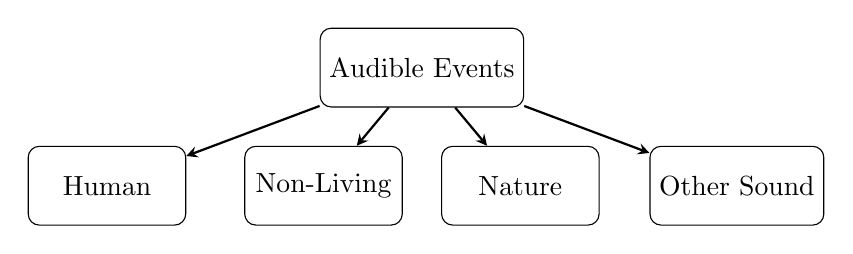
\begin{tikzpicture}[node distance=1.5cm]
		\node (event) [roundRec] {Audible Events}; 
		\node (human) [roundRec, below of=event, xshift=-4cm] {Human}; 
		\node (nonliving) [roundRec, below of=event, xshift=-1.25cm] {Non-Living}; 
		\node (nature) [roundRec, below of=event, xshift=1.25cm] {Nature}; 
		\node (other) [roundRec, below of=event, xshift=4cm] {Other Sound}; 
		\draw [arrow] (event) -- (human);
		\draw [arrow] (event) -- (nonliving);
		\draw [arrow] (event) -- (nature);
		\draw [arrow] (event) -- (other); 
	\end{tikzpicture}
\end{frame}
% ------------------------------------------
\subsection{Audio Data}
\begin{frame}
  \frametitle{Audio Data}	
	We download the audio data for events from Sound Search Engines (SSEs). 
	(List SSEs here)
\end{frame}
% ------------------------------------------
\subsection{Feature Extraction}
\begin{frame}
	\frametitle{Feature Extraction}
	The features we used for training model for audible events are MFCCs. 
\end{frame}
% ------------------------------------------
\subsection{Event Model}
\begin{frame}
	\frametitle{Event Model}	
	We use Gaussian Mixture Models to train the features. 
	(Explain why using GMMs)
\end{frame}
% ------------------------------------------
\section{Scene Recognition}
\subsection{Scene-Event Map}
\begin{frame}
	\frametitle{Script Data}	
	We use the scripts for movies, plays and TV series to extract the scenes. 
\end{frame}
% ------------------------------------------
\begin{frame}
	\frametitle{Scene-Event Relation Mining}
	We calculate the TF-IDF scores for scenes and events. 
\end{frame}
% ------------------------------------------
\subsection{Audio Segmentation}
\begin{frame}
	\frametitle{Audio Segmentation}	
	In testing, we segment the audio into smaller parts for event detection. 
\end{frame}
% ------------------------------------------
\subsection{Scene Inference}
\begin{frame}
	\frametitle{Scene Inference}	
\end{frame}
% ------------------------------------------
\section{Evaluation}
\subsection{Event Detection Evaluation}
\begin{frame}
	\frametitle{Event Detection Evaluation}
\end{frame}
% ------------------------------------------
\subsection{Scene Recognition Evaluation}
\begin{frame}
	\frametitle{Scene Recognition Evaluation}
\end{frame}
% ------------------------------------------
\section{Demo}
\begin{frame}
	\frametitle{Demo}
	Live demo for our system. 
\end{frame}
% ------------------------------------------
%\setbeamertemplate{background canvas}[vertical shading][bottom=white,top=structure.fg!25]
\begin{frame}
  \begin{center}
    {\huge \emph{{Thank  ~you!
          \\   \vspace{1cm} Any Question?}}}
  \end{center}
\end{frame}
\end{document}
